\documentclass[tikz,border=5mm]{standalone}
\usetikzlibrary{calc}

\begin{document}

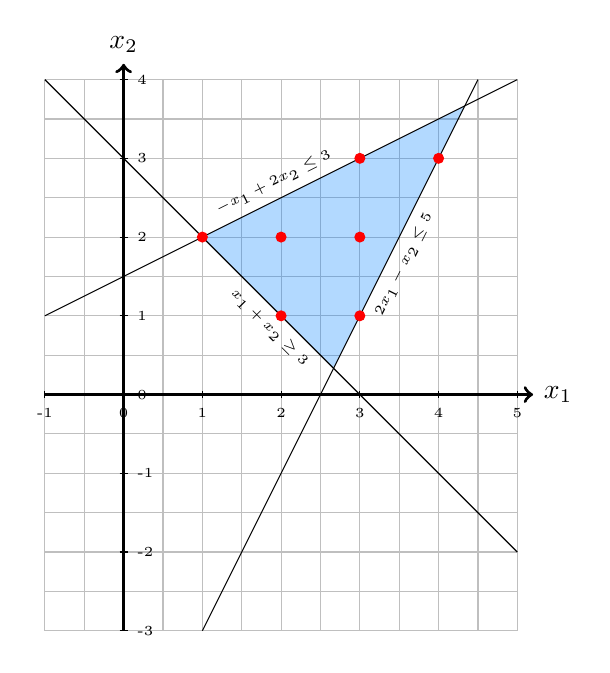
\begin{tikzpicture}

    \draw[gray!50, thin, step=0.5] (-1,-3) grid (5,4);
    \draw[very thick,->] (-1,0) -- (5.2,0) node[right] {$x_1$};
    \draw[very thick,->] (0,-3) -- (0,4.2) node[above] {$x_2$};

    \foreach \x in {-1,...,5} \draw (\x,0.05) -- (\x,-0.05) node[below] {\tiny\x};
    \foreach \y in {-3,...,4} \draw (-0.05,\y) -- (0.05,\y) node[right] {\tiny\y};

    \fill[blue!50!cyan,opacity=0.3] (8/3,1/3) -- (1,2) -- (13/3,11/3) -- cycle;

    \draw (-1,4) -- node[below,sloped] {\tiny$x_1+x_2\geq3$} (5,-2);
    \draw (1,-3) -- (3,1) -- node[below left,sloped] {\tiny$2x_1-x_2\leq5$} (4.5,4);
    \draw (-1,1) -- node[above,sloped] {\tiny$-x_1+2x_2\leq3$} (5,4);



        \fill[red] (2,1) circle(2pt);
        \fill[red] (3,1) circle(2pt);
        \fill[red] (1,2) circle(2pt);
        \fill[red] (2,2) circle(2pt);
        \fill[red] (3,2) circle(2pt);
        \fill[red] (3,3) circle(2pt);
        \fill[red] (4,3) circle(2pt);



\end{tikzpicture}

\end{document}
